\documentclass[tikz,border=2pt]{standalone}
\usepackage{pgfplots}
\pgfplotsset{compat=1.18}
\usetikzlibrary{intersections}
\usepgfplotslibrary{fillbetween}

\begin{document}
	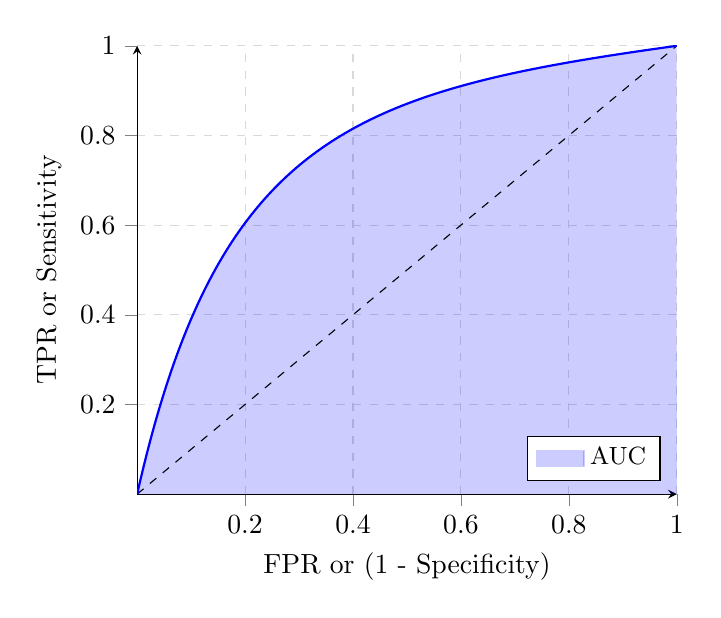
\begin{tikzpicture}
		\begin{axis}[
			axis lines=middle,
			ymin = 0,
			ymax = 1,
			xmin = 0,
			xmax= 1,
			grid = major,
			grid style={dashed, gray!30},
			ylabel near ticks,
			xlabel near ticks,
			xlabel=FPR or (1 - Specificity),
			ylabel=TPR or Sensitivity,
			tick align=outside,
			legend pos= south east,
			legend style={font=\small, cells={align=left}}]
	
	\draw [black, dashed] (0,0) -- (1,1);
	\draw [blue, thick, name path = roc] (0,0) .. controls (0.15,0.8) and (0.4,0.9) .. (1,1);

	\path [name path = axis] (0,0) -- (1,0);


	\addplot [blue, opacity = 0.2] fill between [of = roc and axis, soft clip={domain= 0:1}];
	\addlegendentry{AUC};

		\end{axis}
	\end{tikzpicture} 
\end{document}